
\documentclass[usletter,11pt,english,openany]{article}




\usepackage{float}

%Primary packages
\usepackage{fancyvrb}

\usepackage[utf8]{inputenc}
\usepackage[english]{babel}
\usepackage[pdftex]{graphicx}




% Useful packages:

% Advanced mathematical formulas and symbols
% -------------------------------------
\usepackage{amsmath}
\usepackage{amssymb}
\usepackage{amsfonts}
\usepackage{bm}

% Footnotes
% -------------------------------------
\usepackage[stable,splitrule]{footmisc}

% Color management package
% -------------------------------------
\usepackage[usenames,dvipsnames]{xcolor}

% Control line spacing 
% -------------------------------------
% putting this between footmisc and hyperref seemed to fix broken footnote links
\usepackage{setspace}
\AtBeginDocument{\let~=\nobreakspace}
\spacing{1.4}


\usepackage{lineno}
\linenumbers

\usepackage[bookmarks=true]{hyperref}
\hypersetup{colorlinks=false}
\usepackage{orcidlink}
\usepackage{booktabs}
\usepackage{caption}
\usepackage{longtable}
\usepackage[T1]{fontenc}
\usepackage{geometry}
\geometry{verbose,tmargin=2cm,bmargin=2cm,lmargin=2cm,rmargin=2cm}
\usepackage{array}
\usepackage{url}
\usepackage{multirow}
\usepackage{stackrel}
\usepackage{rotating}


% https://tex.stackexchange.com/questions/151241/remove-metadata-of-pdf-generated-by-latex
\hypersetup{
    bookmarks=true,         % show bookmarks bar?
    unicode=false,          % non-Latin characters in Acrobat's bookmarks
    pdftoolbar=true,        % show Acrobat's toolbar?
    pdfmenubar=true,        % show Acrobat's menu?
    pdffitwindow=false,     % window fit to page when opened
%    pdfstartview={FitW},    % fits the width of the page to the window
    pdftitle={Monero Black Marble Flood},    % title
    pdfauthor={Rucknium},     % author
    pdfsubject={},   % subject of the document
    pdfcreator={Rucknium},   % creator of the document
    pdfproducer={},  % producer of the document
    pdfkeywords={}, % list of keywords
    pdfnewwindow=true,      % links in new window
    colorlinks=false,       % false: boxed links; true: colored links
    linkcolor=red,          % color of internal links
    citecolor=green,        % color of links to bibliography
    filecolor=magenta,      % color of file links
    urlcolor=cyan           % color of external links
}



\begin{document}
\title{March 2024 Suspected Black Marble Flooding Against Monero:
Privacy, User Experience, and Countermeasures\\\vspace{.3cm}
\large Draft v0.2\vspace{-.715cm}}
\author{Rucknium\orcidlink{https://orcid.org/0000-0001-5999-8950} }
\date{March 27, 2024}
\maketitle
\begin{abstract}
On March 4, 2024, aggregate Monero transaction volume suddenly almost
tripled. This note analyzes the effect of the large number of transactions,
assuming that the transaction volume is an attempted black marble
flooding attack by an adversary. According to my estimates, mean effective
ring size has decreased from 16 to 5.5 if the black marble flooding
hypothesis is correct. At current transaction volumes, the suspected
spam transactions probably cannot be used for large-scale ``chain
reaction'' analysis to eliminate all ring members except for the
real spend. Effects of increasing Monero's ring size above 16 are
analyzed.
\end{abstract}

\section{March 4, 2024: Sudden transaction volume }

\begin{figure}[H]
\caption{Volume of Monero transactions with spam fingerprint}
\label{fig-spam-tx-volume}
\centering{}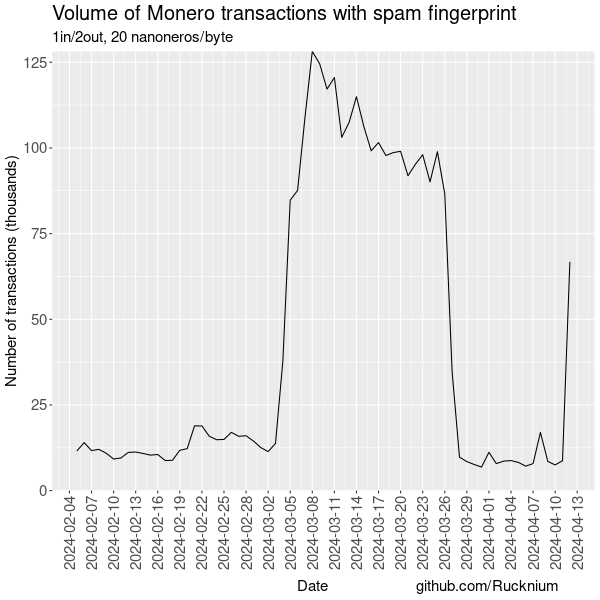
\includegraphics[scale=0.5]{images/spam-fingerprint-tx-volume}
\end{figure}

On March 4, 2024 at approximately block height 3097764 (15:21:24 UTC),
the number of 1input/2output minimum fee (20 nanoneros/byte) transactions
sent to the Monero network rapidly increased. Figure \ref{fig-spam-tx-volume}
shows daily volume of this type of transaction increasing from about
15,000 to over 100,000.

The large volume of these transactions was enough to entirely fill
the 300 kB Monero blocks mined about every two minutes. Monero's dynamic
block size algorithm activated. The 100 block rolling median block
size slowly increased to adjust for the larger number of transactions
that miners could pack in blocks. Figure \ref{fig-empirical-block-weight}
shows the adjustment. The high transaction volume raised the 100 block
median gradually for period of time. Then the transaction volume reduced
just enough to allow the 100 block median to reset to a lower level.
Then the process would restart. Block sizes have usually remained
between 300 kB and 400 kB. Occasionally, high-fee transactions would
allow miners to get more total revenue by giving up some of the 0.6
XMR/block tail emission and including more transactions in a block.
The ``maximum peaks'' plot shows this phenomenon.

\begin{figure}[H]
\caption{Monero empirical block weight}
\label{fig-empirical-block-weight}
\centering{}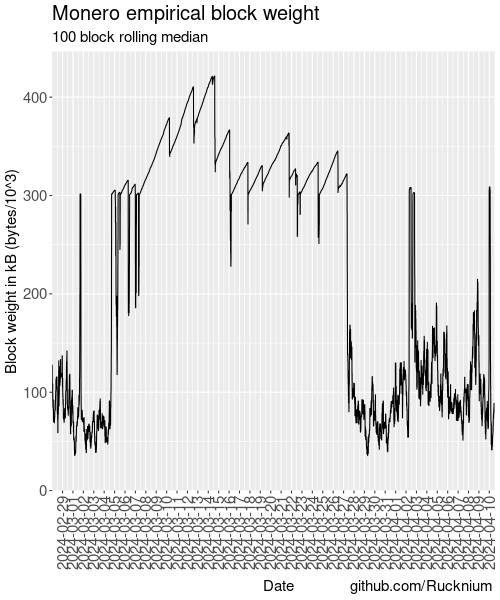
\includegraphics[scale=0.5]{images/rolling-median-block-weight}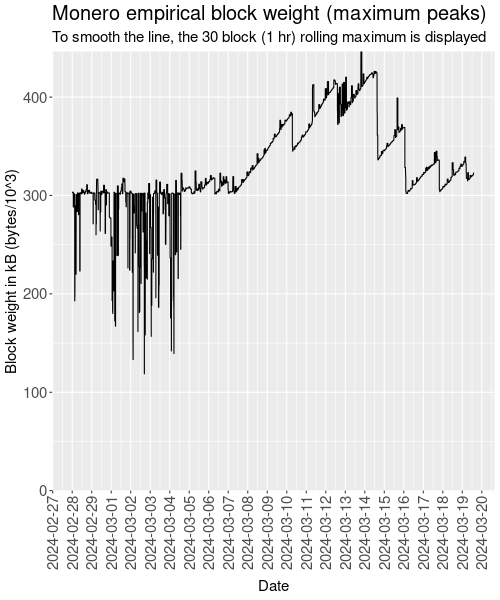
\includegraphics[scale=0.5]{images/rolling-max-block-weight}
\end{figure}

The sudden transaction volume rise may originate from a single entity.
The motive may be spamming transactions to bloat the blockchain size,
increase transaction confirmation times for real users, perform a
network stress test, or execute a black marble flooding attack to
reduce the privacy of Monero users. I will focus most of my analysis
on the last possibility.

\section{Literature review}

The very first research bulletin released by the Monero Research Lab
described black marble transaction flooding. \cite{Noether2014} points
out that the ring signature privacy model requires rings to contain
transaction outputs that are could be plausible real spends. If a
single entity owns a large share of outputs (spent or not), it can
use its knowledge to rule out ring members in other users' transactions
that cannot be the real spend. Since the entity knows that itself
did not spend the output(s) in a particular ring, the effective ring
size that protects other users' privacy can be reduced --- even to
an effective ring size of 1 when the entity knows the real spend with
certainty. Rings with known real spends can be leveraged to determine
the real spend in other rings in a ``chain reaction'' attack.

\cite{Noether2014} gave the name ``black marble'' to the outputs
owned by an anti-privacy adversary since they modeled the problem
using a marble draw problem with a hypergeometric distribution. When
a specific number of marbles are drawn \textit{without} replacement
from an urn containing a specific number of white and black marbles,
the hypergeometric distribution describes the probability of drawing
a specific number of black marbles. In my modeling I use the binomial
distribution, which is the same as the hypergeometric except marbles
are drawn \textit{with} replacement. The binomial distribution makes
more sense now ten years after \cite{Noether2014} was written. The
total number of RingCT outputs on the blockchain that can be included
in a ring is over 90 million. The hypergeometric distribution converges
to the binomial distribution as the total number of marbles increases
to infinity. Moreover, Monero's current decoy selection algorithm
does not select all outputs with equal probability. More recent outputs
are selected with much higher probability. The hypergeometric distribution
cannot be used when individual marbles have unequal probability of
being selected.

\cite{Chervinski2021} simulates a realistic black marble flood attack.
They consider two scenarios. The adversary could create 2input/16output
transactions to maximize the number of black marble outputs per block
or the adversary could create 2input/2output transactions to make
the attack less obvious. The paper uses Monero transaction data from
2020 to set the estimated number of real outputs and kB per block
at 41 outputs and 51 kB respectively. The nominal ring size at this
time was 11. The researchers simulated filling the remaining 249 kB
of the 300 kB block with black marble transactions. A ``chain reaction''
algorithm was used to boost the effectiveness of the attack. In the
2in/2out scenario, the real spend could be deduced (effective ring
size 1) in 11\% of rings after one month of spamming black marbles.
Later I will compare the results of this simulation with the current
suspected spam incident.

\cite{Krawiec-Thayer2021} analyze a suspected spam incident in July-August
2021. Transactions' inputs, outputs, fees, and ring member ages were
plotted to evaluate evidence that a single entity created the spam.
The analysis concluded, ``All signs point towards a single entity.
While transaction homogeneity is a strong clue, a the {[}sic{]} input
consumption patterns are more conclusive. In the case of organic growth
due to independent entities, we would expect the typically semi-correlated
trends across different input counts, and no correlation between independent
users\textquoteright{} wallets. During the anomaly, we instead observed
an extremely atypical spike in 1--2 input txns with no appreciable
increase in 4+ input transactions.''

TODO: A few papers like \cite{Ronge2021,Egger2022} discuss black
marble attacks too.

\section{Black marble theory}

The binomial distribution describes the probability of drawing $x$
number of ``successful'' items when drawing a total of $n$ items
when the probability of a successful draw is $p$. It can be used
to model the number of transaction outputs selected by the decoy selection
algorithm that are not controlled by a suspected adversary.

The probability mass function of the binomial distribution with $n\in\{0,1,2,\ldots\}$
number of draws and $p\in[0,1]$ probability of success is

\begin{equation}
f(x,n,p)=\binom{n}{x}p^{x}\left(1-p\right)^{n-x}\textrm{, where }\binom{n}{x}=\frac{n!}{x!(n-x)!}
\end{equation}

The expected value (the theoretical mean) of a random variable with
a binomial distribution is $np$.

Monero's standard decoy selection algorithm programmed in \texttt{wallet2}
does not select outputs with equal probability. The probability of
selecting each output depends on the age of the output. Specifics
are in \cite{Rucknium2023a}. The probability of a single draw selecting
an output that is not owned by the adversary, $p_{r}$, is equal to
the share of the probability mass function occupied by those outputs:
$p_{r}=\sum_{i\in R}g(i)$, where $R$ is the set of outputs owned
by real users and $g(x)$ is the probability mass function of the
decoy selection algorithm.

\subsection{Spam assumptions\label{subsec:spam-assumptions}}

There is some set of criteria that identifies suspected spam. The
early March 2024 suspected spam transactions: 1) have one input; 2)
have two outputs; 3) pay the minimum 20 nanoneros per byte transaction
fee. The normal volume of these transactions produced by real users
must be estimated. The volume in excess of the normal volume is assumed
to be spam. I followed this procedure:
\begin{enumerate}
\item Compute the mean number of daily transactions that fit the suspected
spam criteria for the four weeks that preceded the suspected spam
incident. A separate mean was calculated for each day of the week
(Monday, Tuesday,...) because Monero transaction volumes have weekly
cycles. These volume means are denoted $v_{r,m},v_{r,t},v_{r,w},\ldots$
for the days of the week.
\item For each day of the suspected spam interval, sum the number of transactions
that fit the suspected spam criteria. Subtract the amounts found in
step (1) from this sum, matching on the day of the week. This provides
the estimated number of spam transactions for each day: $v_{s,1},v_{s,2},v_{s,3},\ldots$
\item For each day of the suspected spam interval, randomly select $v_{s,t}$
transactions from the set of transactions that fit the suspected spam
criteria, without replacement. This randomly selected set is assumed
to be the true spam transactions.
\item During the period of time of the spam incident, compute the expected
probability $p_{r}$ that one output drawn from the \texttt{wallet2}
decoy distribution will select an output owned by a real user (instead
of the adversary) when the wallet constructs a ring at the point in
time when the blockchain tip is at height $h$. The closed-form formula
of the \texttt{wallet2} decoy distribution is in \cite{Rucknium2023a}.
\item The expected effective ring size of each ring constructed at block
height $h$ is $1+15\cdot p_{r}$. The coefficient on $p_{r}$ is
the number of decoys.
\end{enumerate}
Figure \ref{fig-estimated-mean-effective-ring-size} shows the results
of this methodology. The mean effective ring size settled at about
5.5 by the fifth day of the large transaction volume. On March 12
and 13 there was a large increase in the number of 1input/2output
transactions that paid 320 nanoneros/byte (the third fee tier). This
could have been the spammer switching fee level temporarily or a service
that uses Monero increasing fees to avoid delays. I used the same
method to estimate the spam volume of these 320 nanoneros/byte suspected
spam. The 1in/2out 320 nanoneros/byte transactions displaced some
of the 1in/2out 20 nanoneros/byte transactions because miners preferred
to put transactions with higher fees into blocks. Other graphs and
analysis will consider only the 1in/2out 20 nanoneros/byte transactions
as spam unless indicated otherwise.

\begin{figure}[H]
\caption{Estimated mean effective ring size}
\label{fig-estimated-mean-effective-ring-size}
\centering{}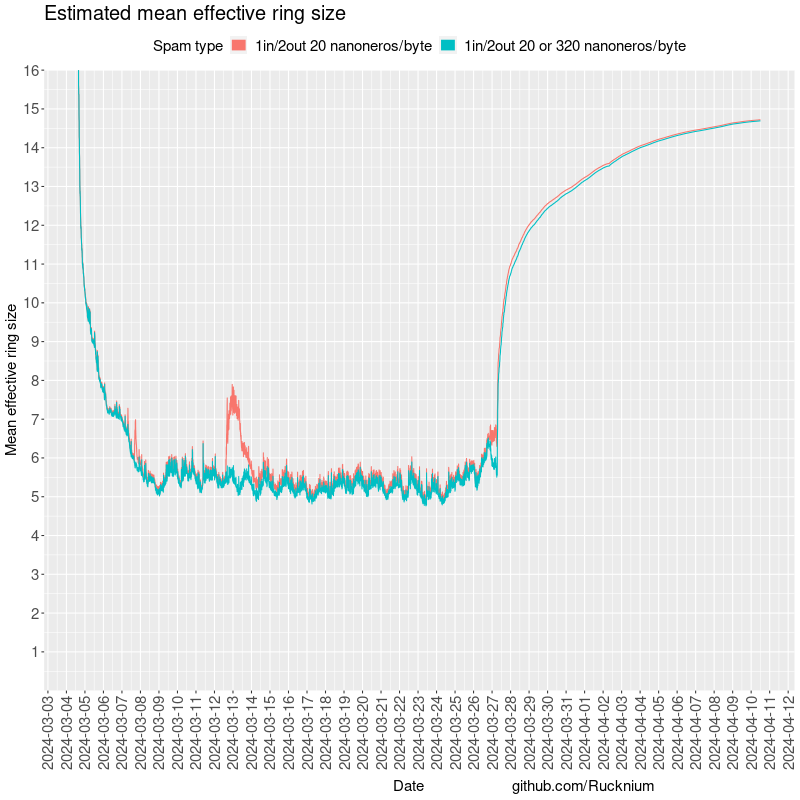
\includegraphics[scale=0.5]{images/empirical-effective-ring-size}
\end{figure}

Figure \ref{fig-spam-share-outputs} shows the daily share of outputs
on the blockchain that are owned by the suspected spammer. The mean
share of outputs since the suspected spam started is about 75 percent.

\begin{figure}[H]
\caption{Spam share of outputs}
\label{fig-spam-share-outputs}
\centering{}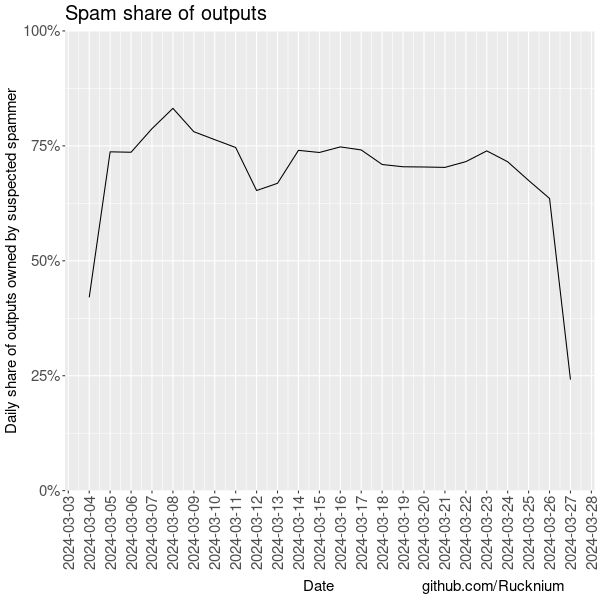
\includegraphics[scale=0.5]{images/spam-share-outputs}
\end{figure}


\subsection{Long term projection scenarios at different ring sizes}

Fix the number of outputs owned by real users at $r$. The analysis
will let the number $s$ of outputs owned by the adversary vary. The
share of outputs owned by real users is

\begin{equation}
p_{r}=\dfrac{r}{r+s}\label{eq:p_r-fixed-real}
\end{equation}

The \ref{eq:p_r-fixed-real} expression can be written $p_{r}=\frac{1}{r}\cdot\dfrac{r}{1+\tfrac{1}{r}s}$
, which is the formula for hyperbolic decay with the additional $\frac{1}{r}$
coefficient at the beginning of the expression \cite{Aguado2010}.

Let $n$ be the nominal ring size (16 in Monero version 0.18). The
number of decoys chosen by the decoy selection algorithm is $n-1$.
The mean effective ring size for a real user's ring is one (the real
spend) plus the ring's expected number of decoys owned by other real
users.

\begin{equation}
\mathrm{E}\left[n_{e}\right]=1+\left(n-1\right)\cdot\dfrac{r}{r+s}\label{eq:expectation-n_e}
\end{equation}

The empirical analysis of Section \ref{subsec:spam-assumptions} considered
the fact that the \texttt{wallet2} decoy selection algorithm draws
a small number of decoys from the pre-spam era. Now we will assume
that the spam incident has continued for a very long time and all
but a negligible number of decoys are selected from the spam era.
We will hold constant the non-spam transactions and vary the number
of spam transactions and the ring size. Figures \ref{fig-projected-effective-ring-size-non-log},
\ref{fig-projected-effective-ring-size-log-log}, and \ref{fig-projected-share-ring-size-one}
show the results of the simulations.

\begin{figure}[H]
\caption{Long-term projected mean effective ring size}
\label{fig-projected-effective-ring-size-non-log}
\centering{}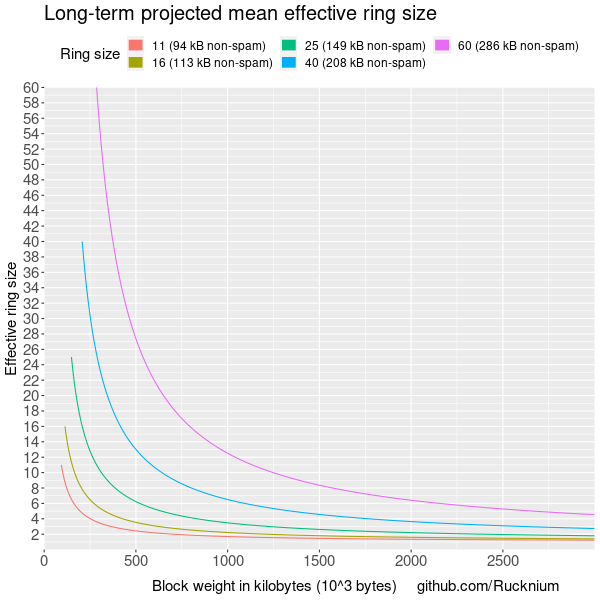
\includegraphics[scale=0.5]{images/projected-effective-ring-size-non-log}
\end{figure}

\begin{figure}[H]
\caption{Long-term projected mean effective ring size (log-log scale)}
\label{fig-projected-effective-ring-size-log-log}
\centering{}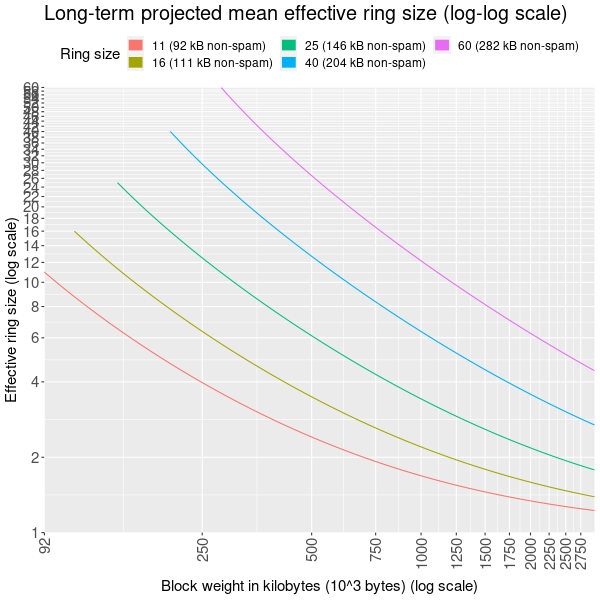
\includegraphics[scale=0.5]{images/projected-effective-ring-size-log-log}
\end{figure}

\begin{figure}[H]
\caption{Long-term projected share of rings with effective ring size 1}
\label{fig-projected-share-ring-size-one}
\centering{}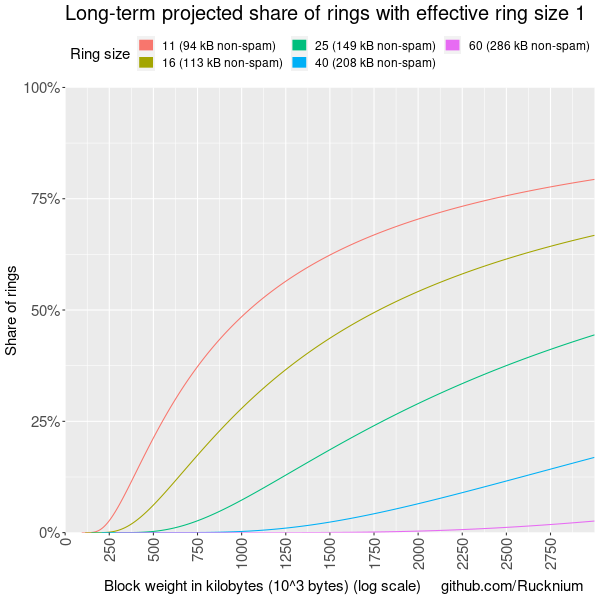
\includegraphics[scale=0.5]{images/projected-ring-size-one}
\end{figure}


\subsection{Guessing the real spend using a black marble flooder's simple classifier}

The adversary carrying out a black marble flooding attack could use
a simple classifier to try to guess the real spend: Let $n$ be nominal
ring size and $n_{s}$ be the number of outputs in a given ring that
are owned by the attacker. $n_{s}$ is a random variable because decoy
selection is a random process. The adversary can eliminate $n_{s}$
of the $n$ ring members as possible real spends. The attacker guesses
randomly with uniform probability that the $i$th ring member of the
$n-n_{s}$ remaining ring members is the real spend. The probability
of correctly guessing the real spend is $\frac{1}{n-n_{s}}$. If the
adversary owns all ring members except for one ring member, which
must be the real spend, the probability of correctly guessing the
real spend is 100\%. If the adversary owns all except two ring members,
the probability of correctly guessing is 50\%. And so forth.

The mean effective ring size is $\mathrm{E}\left[n_{e}\right]$ from
\ref{eq:expectation-n_e}. Does this mean that the mean probability
of correctly guessing the real spend is $\frac{1}{\mathrm{E}\left[n_{e}\right]}$?
No. The $h(x)=\frac{1}{x}$ function is strictly convex. By Jensen's
inequality, $\mathrm{E}\left[\frac{1}{n_{e}}\right]>\frac{1}{\mathrm{E}\left[n_{e}\right]}$.
The mean probability of correctly guessing the real spend is

\begin{equation}
\mathrm{E}\left[\frac{1}{n_{e}}\right]=\stackrel[i=1]{n}{\sum}\dfrac{1}{i}\cdot f(i-1,n-1,\frac{\mathrm{E}\left[n_{e}\right]-1}{n-1})
\end{equation}

$\frac{1}{i}$ is the probability of correctly guessing the real spend
when the effective ring size is $i$. $f$ is the probability mass
function of the binomial distribution. It calculates the probability
of the decoy selection algorithm selecting $i-1$ decoys that are
owned by real users. The total number of decoys to select is $n-1$
(that is the argument in the second position of $f$). The probability
of selecting a decoy owned by a real user is $\frac{\mathrm{E}\left[n_{e}\right]-1}{n-1}=\frac{r}{r+s}$.

\begin{figure}[H]
\caption{Estimated probability of correctly guessing the real spend}
\label{fig-prob-guessing-real-spend}
\centering{}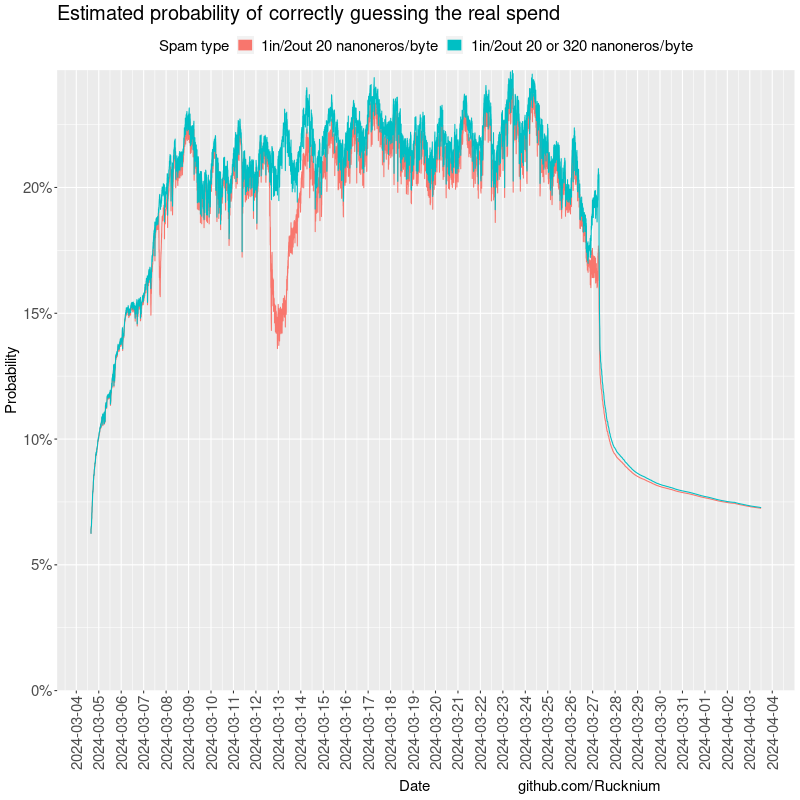
\includegraphics[scale=0.5]{images/empirical-guessing-probability}
\end{figure}

The probability of a given ring having all adversary-owned ring members
except for the real spend is $f\left(0,n-1,\frac{\mathrm{E}\left[n_{e}\right]-1}{n-1}\right)$
. Figure \ref{fig-share-ring-size-one} plots the estimated share
of rings with effective ring size one.

\begin{figure}[H]
\caption{Estimated share of rings with effective ring size of one}
\label{fig-share-ring-size-one}
\centering{}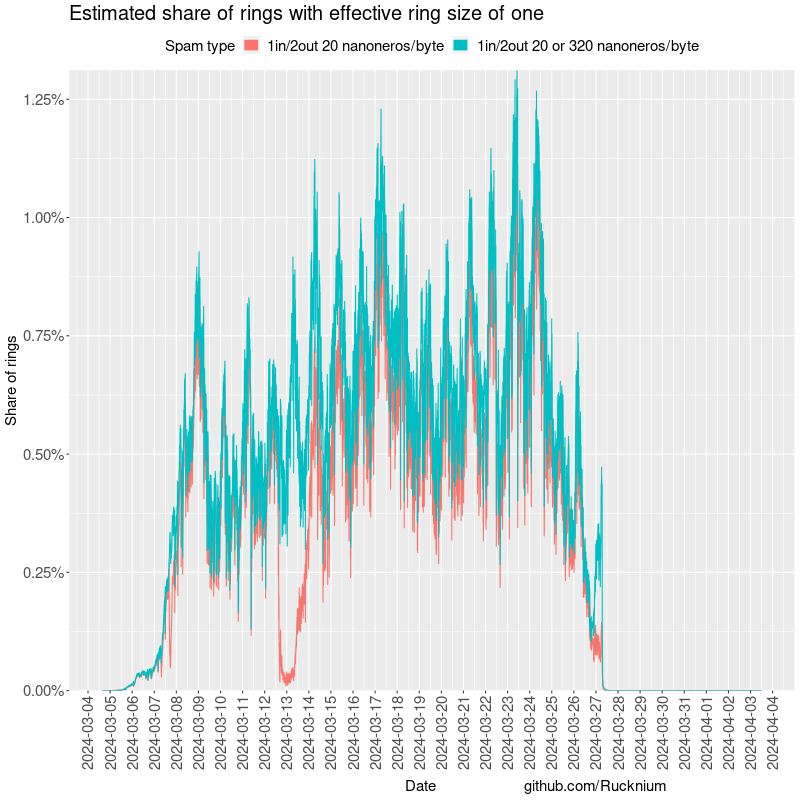
\includegraphics[scale=0.5]{images/empirical-ring-size-one}
\end{figure}


\section{Chain reaction graph attacks}

The effective ring size can be reduced further by applying a process
of elimination to related rings. This technique is called a ``chain
reaction'' or a ``graph analysis attack''. Say that the effective
ring size in transaction $A$ is reduced to two because of a black
marble attack. One of the remaining two ring members is an output
in transaction $B$. If the output in transaction $B$ is known to
be spent in transaction $C$ because the effective ring size of transaction
$C$ was one, then that output can be ruled out as a plausible real
spend in transaction $A$. Therefore, the adversary can reduce the
effective ring size of transaction $A$ to one.

Theorem 1 of \cite{Yu2019a} says that a ``closed set'' attack is
as effective as exhaustively checking all subsets of outputs. The
brute force attack is infeasible since its complexity is $O\left(2^{m}\right)$,
where $m$ is the total number of RingCT outputs on the blockchain.
\cite{Yu2019a} implements a heuristic algorithm to execute the closed
set attack that is almost as effective as the brute force method.
\cite{Vijayakumaran2023} proves that the Dulmage-Mendelsohn (DM)
decomposition gives the same results as the brute force closed set
attack, but the algorithm renders a result in polynomial time. The
open source implementation of the DM decomposition in \cite{Vijayakumaran2023}
processes 37 million RingCT rings in about four hours.

In practice, how much further can chain reaction attacks reduce the
effective ring size when combined with a black marble attack? \cite{Egger2022}
suggest some closed-form formulas to compute the vulnerability of
different ring sizes to chain reaction attacks. However, \cite{Egger2022}
assume that decoys are selected by a partitioning process instead
of Monero's actual mimicking decoy selection algorithm. It is not
clear how relevant the findings of \cite{Egger2022} are for Monero's
mainnet. Monte Carlo simulations would be a better way to evaluate
the risk of chain reactions.

\cite{Chervinski2021} carries out a simulation using the old ring
size of 11. In the 2input/2output spam scenario, 82\% of outputs are
black marbles. Assuming only the binomial distribution, i.e. no chain
reaction analysis, Figure \ref{fig-effective-ring-size-binomial-pmf}
compares the theoretical long-term distribution of effective ring
sizes in the \cite{Chervinski2021} scenario and the March 2024 suspected
spam on Monero's mainnet. The share of rings with effective ring size
1 in the \cite{Chervinski2021} scenario is 11.9 percent, but the
share is only 0.8 percent with the suspected March 2024 spam. The
mean effective ring sizes of the \cite{Chervinski2021} scenario without
chain reaction and the March 2024 spam estimate are 2.9 and 5.2, respectively.

\begin{figure}[H]
\caption{Probability mass function of long-term effective ring sizes}
\label{fig-effective-ring-size-binomial-pmf}
\centering{}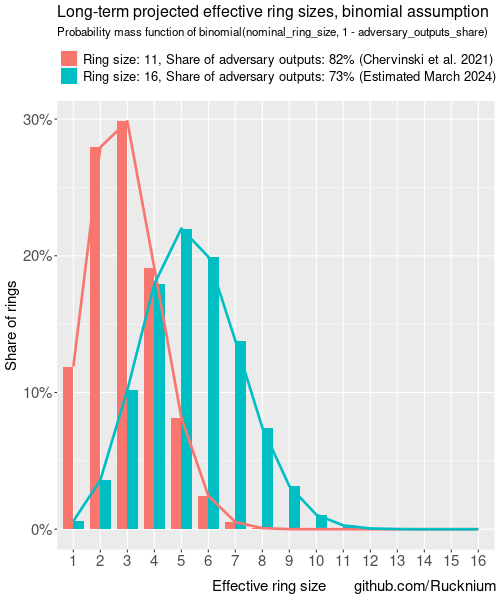
\includegraphics[scale=0.5]{images/effective-ring-size-binomial-pmf}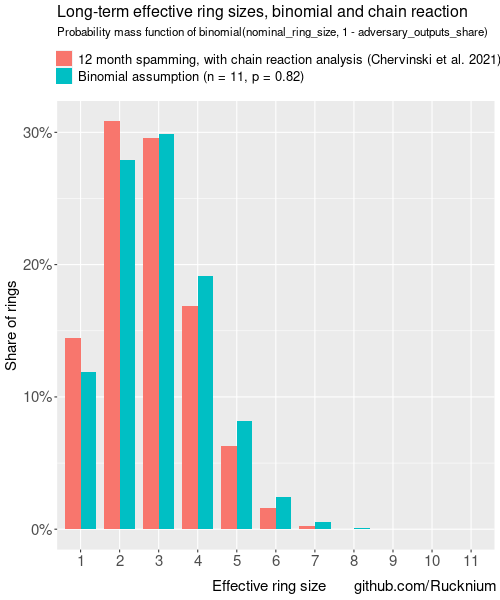
\includegraphics[scale=0.5]{images/chervinski-chain-reaction}
\end{figure}

\cite{Chervinski2021} executes chain reaction analysis to increase
the effectiveness of the attack. The second plot in Figure \ref{fig-effective-ring-size-binomial-pmf}
compares the long term effective ring size achieved by \cite{Chervinski2021}
when leveraging chain reaction analysis and the effective ring size
when only the binomial distribution is assumed. \cite{Chervinski2021}
increases the share of ring with effective ring size one from 11.9
to 14.5 percent. Mean effective ring size decreases from 2.94 to 2.76.
This is a modest gain of attack effectiveness, but \cite{Chervinski2021}
appears to be using a suboptimal chain reaction algorithm instead
of the closed set attack.

The actual risk from chain reaction analysis in the suspected March
2024 flooding is a gap in our knowledge. \cite{Vijayakumaran2023}
provides an open source implementation of the DM decomposition in
Rust and excellent documentation.\footnote{\url{https://github.com/avras/cryptonote-analysis}\\
\url{https://www.respectedsir.com/cna}} A Monte Carlo simulation applying the DM decomposition to the March
2024 black marble estimates should be written.

\section{Countermeasures}

See \url{https://github.com/monero-project/research-lab/issues/119}

TODO

\section{Estimated cost to suspected spammer}

When the 1in/2out 20 nanoneros/byte spam definition is used, the total
fees paid by the spam transactions over the 23 days of spam was 61.5
XMR. The sum total of the transaction sizes of the spam transactions
was 3.08 GB.

When the 1in/2out 20 or 320 nanoneros/byte spam definition is used,
the total fees paid by the spam transactions over the 23 days of spam
was 81.3 XMR. The sub total of the transaction sizes of the spam transactions
was 3.12 GB.

\section{Transaction confirmation delay}

Monero's transaction propagation rules are different from BTC's rules
for good reasons, but two of the rules can make transactions seem
like they are ``stuck'' when the txpool (mempool) is congested.
First, Monero does not have replace-by-fee (RBF). When a Monero node
sees that a transaction attempts to spend an output that is already
spent by another transaction in the txpool, the node does not send
the transaction to other nodes because it is an attempt to double
spend the output. (Monero nodes do not know the real spend in the
ring, but double spends can be detected by comparing the key images
of ring signatures in different transactions.) Monero users cannot
increase the fee of a transaction that they already sent to a node
because the transaction with the higher fee would be considered a
double spend. BTC has RBF that allows a transaction to replace a transaction
in the mempool that spends the same output if the replacement transaction
pays a higher fee. One of RBF's downsides is that merchants cannot
safely accept zero-confirmation transactions because a malicious customer
can replace the transaction in the mempool with a higher-fee transaction
that spends the output back to themselves. Without RBF, Monero users
must wait for their low-fee transaction to confirm on the blockchain.
They cannot choose to raise their ``bid'' for block space even if
they were willing to pay more. They have to get it right the first
time. Fee prediction is especially important for Monero users when
the txpool is congested because of the lack of RBF, but very little
Monero-specific fee prediction research has been done.

Unlike BTC, Monero also does not have child-pays-for-parent (CPFP),
which allows users to chain multiple transactions together while they
are still in the mempool. With CPFP, users can spend the output of
the unconfirmed parent transaction and attach a higher fee to the
child transaction. Miners have an incentive to include the parent
transaction in the block because the child transaction is only valid
if the parent transaction is also mined in a block. Monero transaction
outputs cannot be spent in the same block that they are confirmed
in. Actually, Monero users need to wait at least ten blocks to spend
new transaction outputs because benign or malicious blockchain reorganizations
can invalidate ring signatures.\footnote{``Eliminating the 10-block-lock'' \url{https://github.com/monero-project/research-lab/issues/95}}

Monero's transaction propagation rules can create long delays for
users who pay the same minimum fee that the suspected spammer pays.
When users pay the same fee as the spam, their transactions are put
in a ``queue'' with other transactions at the same fee per byte
level. Their transactions are confirmed in first-in/first-out order
because the \texttt{get\_block\_template} RPC call to \texttt{monerod}
arranges transactions that way.\footnote{\url{https://github.com/monero-project/monero/blob/9bf06ea75de4a71e3ad634e66a5e09d0ce021b67/src/cryptonote_core/tx_pool.cpp\#L1596}}
Most miners use \texttt{get\_block\_template} to construct blocks,
but P2Pool orders transactions randomly after they have been sorted
by fee per byte.\footnote{\url{https://github.com/SChernykh/p2pool/blob/dd17372ec0f64545311af40b976e6274f625ddd8/src/block_template.cpp\#L194}}

The first plot in Figure \ref{fig-delay-tx-confirmation} shows the
mean delay of transaction confirmation in each hour. The plot shows
the mean time that elapsed between when the transaction entered the
txpool and when it was confirmed in a block. Each hour's value in
the line plot is computed from transactions that were confirmed in
blocks in that hour. This data is based on txpool archive data actively
collected from a few nodes.\footnote{\url{https://github.com/Rucknium/misc-research/tree/main/Monero-Mempool-Archive}}
The mean includes transactions with and without the spam fingerprint.
Usually mean confirmation time was less than 30 minutes, but sometimes
confirmations of the average transaction were delayed by over two
hours.

\begin{figure}[H]
\caption{Delay to first transaction confirmation}
\label{fig-delay-tx-confirmation}
\centering{}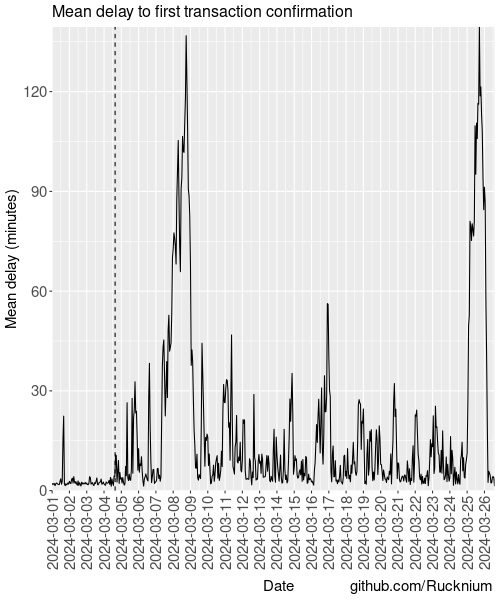
\includegraphics[scale=0.5]{images/mean-delay-first-confirmation}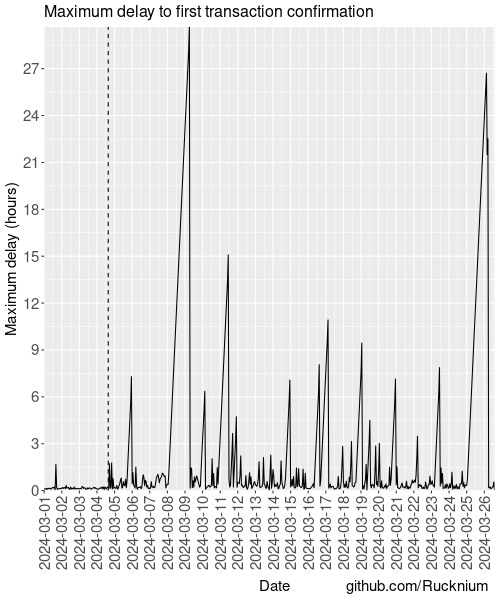
\includegraphics[scale=0.5]{images/max-delay-first-confirmation}
\end{figure}

The second plot in Figure \ref{fig-delay-tx-confirmation} shows the
\textit{maximum} waiting time for a transaction to be confirmed. The
value of the line at each hour is the longest time that a transaction
waited to be confirmed in one of the block mined in the hour or the
amount of time that a transaction was still waiting to be confirmed
at the end of the hour (whichever is greater). There were a handful
of transactions that paid fees below the 20 nanoneros/byte tier that
the spam was paying. These transactions did not move forward in the
queue when the spam transactions were confirmed. Instead, they had
to wait until the txpool completely emptied. Exactly 100 transactions
waited longer than three hours. They paid between 19465 and 19998
piconeros per byte. Most of the transactions appeared to have set
fees slightly lower than 20 nanonerpos per byte because they had an
unusual number of inputs. 92 of them had four or more inputs. The
remaining eight of them had just one input. Those eight may have been
constructed by a nonstandard wallet.

\section{Real user fee behavior}

During the suspected spam, users must pay more than the minimum fee
to put their transactions at the front of the confirmation queue.
If users pay more than the minimum fee, usually their transactions
would be confirmed in the next mined block. Monero's standard fee
levels are 20, 80, 320, and 4000 nanoneros per byte. Users are not
required to pay one of these fee levels, but all wallets that are
based on \texttt{wallet2} do not allow users to choose custom fees
outside of the four standard levels because of the privacy risk of
unusual transactions.\footnote{\url{https://github.com/Rucknium/misc-research/tree/main/Monero-Nonstandard-Fees}}

The ``auto'' fee level of the Monero GUI and CLI wallets is supposed
to automatically change the fee of a transaction from the lowest tier
(20 nanoneros/byte) to the second tier (80 nanoneros/byte) when the
txpool is congested. Unfortunately, a bug prevented the automatic
adjustment. On March 9, 2024 the Monero Core Team released the 0.18.3.2
version of Monero and the GUI/CLI wallet that fixed the bug.\footnote{``Monero 0.18.3.2 'Fluorine Fermi' released'' \url{https://www.getmonero.org/2024/03/09/monero-0.18.3.2-released.html}

``wallet2: adjust fee during backlog, fix set priority'' \url{https://github.com/monero-project/monero/pull/9220}} Users are not required to upgrade to the latest wallet version, so
probably many users still use the version that is not automatically
adjusting fees.

The first plot of Figure \ref{fig-share-tx-by-fee-tier} shows the
share of trasnactions paying each of the four fee tiers. Any transactions
that do not pay in the standard ranges $\left\{ \left[18,22\right],\left[72,82\right],\left[315,325\right],\left[3000,4100\right]\right\} $
were not included in the plot. The 320 nanoneros/byte tier is interesting.
About 10 percent of transactions paid 320 nanonero/byte until Februray
17, 2024. The date could have something to do with Monero being delisted
from Binance on February 20, 2024.\footnote{\url{https://decrypt.co/218194/binance-finalizes-monero-delisting}}
Then on March 12-13, 2024 there was a burst of 320 nanonero/byte transactions.
The 0.18.3.2 GUI/CLI wallet release could not explain the burst since
the auto fee adjustment would only increase fees from 20 to 80 nanoneros/byte.
The burst of 320 nanonero/byte transactions must have been either
from a central service producing fees or from the suspected spammer.

The second plot of Figure \ref{fig-share-tx-by-fee-tier} shows the
same data with the suspected spam transactions eliminated both the
80 and 320 nanoneros/byte transactions with the spam fingerprint were
removed. There is a modest increase in 80 nanonero/byte transactions
after the spam started.

\begin{figure}[H]
\caption{Share of transactions by fee tier}
\label{fig-share-tx-by-fee-tier}
\centering{}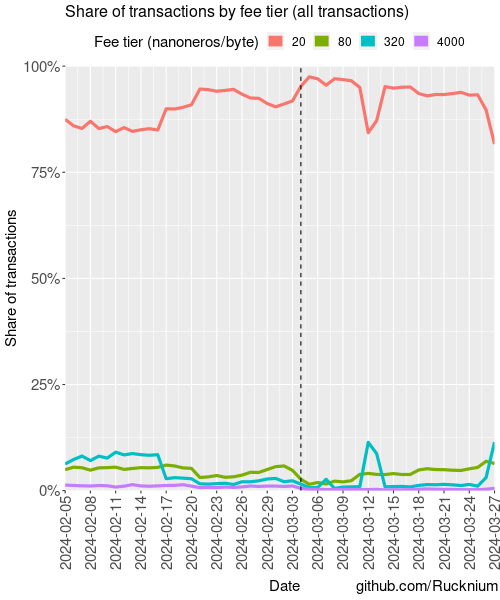
\includegraphics[scale=0.5]{images/share-tx-in-fee-tier-all-txs}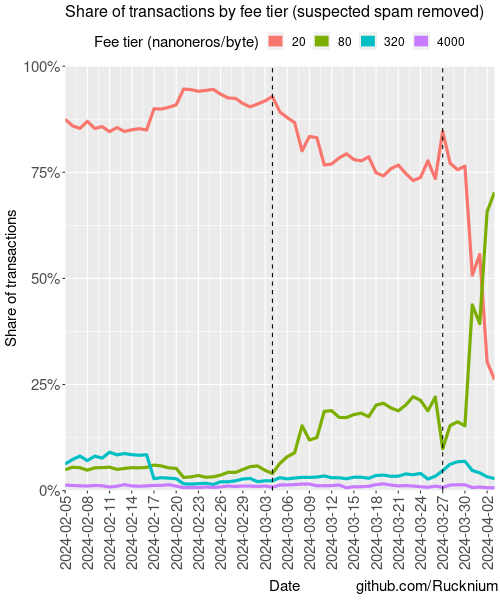
\includegraphics[scale=0.5]{images/share-tx-in-fee-tier-spam-removed}
\end{figure}

The mempool archive data suggest that merchants using zero-confirmation
delivery were still safe during the spam incident. Once submitted
to the network, transactions did not drop out of the mempool. They
just took longer to confirm. There were only two transaction IDs in
the mempool of one of the mempool archive nodes that did not confirm
during the spam period. Both occurred on March 8 when the mempool
was very congested. The the two ``disappearing transactions'' could
happen if someone submits a transactions to an overloaded public RPC
node, the transactions does not propagate well, and then the user
reconstructs the transactions with another node. The first transaction
will not confirm because it is a double spend. Seeing a transaction
in the mempool that never confirms happens sometimes during normal
transaction volumes, too. Single transactions like that appeared on
February 14, 17, and 23 and March 1 in the mempool archive data.

\section{Evidence for and against the spam hypothesis}

Is the March 4, 2024 transaction volume a result of many real users
starting to use Monero more, or is it spam created by a single entity?
\cite{Krawiec-Thayer2021} analyzed the July/August 2021 sudden rise
in transaction volume. We concluded that it was likely spam. Our evidence
was: 1) There was a sharp increase of 1in/2out and 2in/1out transactions,
but the volume of other transaction types did not increase, 2) All
the suspected spam paid minimum fees, 3) The distribution of ring
members became much younger, suggesting that the spammer was rapidly
re-spending outputs as quickly as possible.

Available time has not permitted a full run of the \cite{Krawiec-Thayer2021}
analysis on the March 2024 suspected spam data. It is easy to do a
quick check of transaction volume by input/output type. Figure \ref{fig-in-out-tx-type-volume}
plots the eight most common in/out transaction types on a log scale.
Only the volume of 1in/2out transactions increased on March 4, supporting
the spam hypothesis.

\begin{figure}[H]
\caption{Transaction volume by number of inputs and outputs (log scale)}
\label{fig-in-out-tx-type-volume}
\centering{}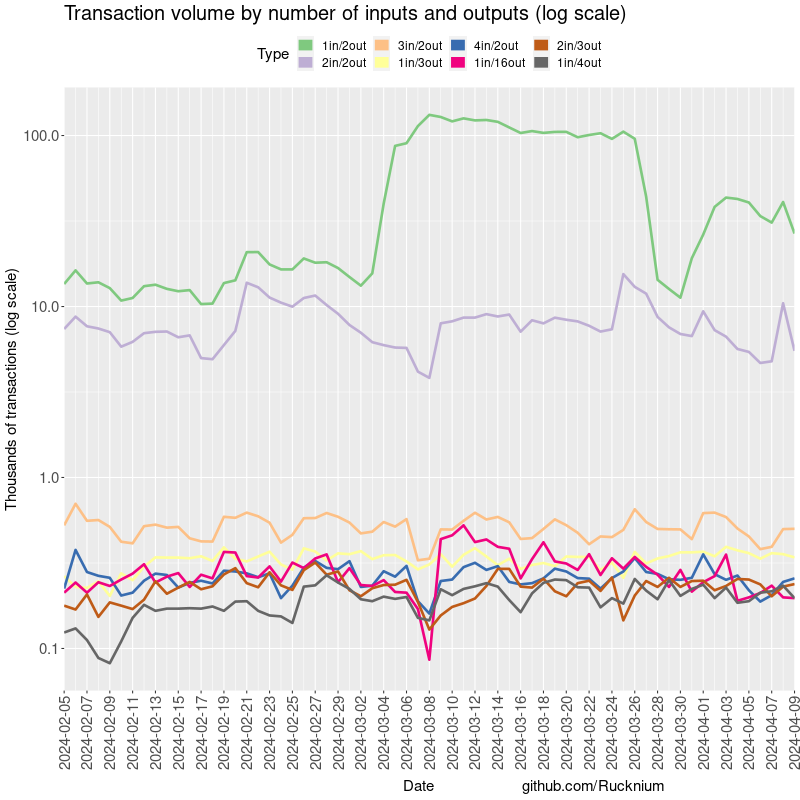
\includegraphics[scale=0.5]{images/in-out-tx-type-volume}
\end{figure}

More can be done to generate evidence for or against the spam hypothesis.
\cite{Krawiec-Thayer2021} analyzed the age of all ring members. Using
the OSPEAD techniques, the distribution of the age of the real spends
can be estimated.\footnote{\url{https://github.com/Rucknium/OSPEAD}}
The Monero node network can be actively crawled to see if the spam
transactions originate from one node. Dandelion++ can defeat attempts
to discover the origin of most transaction because the signal of the
real transaction is covered by the Dandelion++ noise. When the signal
is huge like the spam, some statistical analysis could overcome the
Dandelion++ protection. Investigatory nodes could use \texttt{set\_log
net.p2p.msg:INFO} to view which neighboring nodes the suspected spam
is coming from. Then the investigatory node could crawl the network
in the direction of the highest incoming volume. The techniques of
\cite{Sharma2022} are useful at extremely high transaction volumes,
like in the spam case, and could be used.

\bibliographystyle{apalike-ejor}
\bibliography{monero-black-marble-flood}

\end{document}
